\documentclass[aps,twocolumn,twoside,secnumarabic,balancelastpage,amsmath,amssymb,nofootinbib,hyperref=pdftex]{revtex4}

\usepackage[utf8]{inputenc}
\usepackage{siunitx}
\usepackage{chapterbib}    % allows a bibliography for each chapter (each labguide has it's own)
\usepackage{color}         % produces boxes or entire pages with colored backgrounds
\usepackage{graphics}      % standard graphics specifications
\usepackage[pdftex]{graphicx}      % alternative graphics specifications
\usepackage{longtable}     % helps with long table options
\usepackage{epsf}          % old package handles encapsulated post script issues
\usepackage{bm}            % special 'bold-math' package
\usepackage{verbatim}			% for comment environment
%\usepackage{asymptote}     % For typesetting of mathematical illustrations
%\usepackage{thumbpdf}
\usepackage[colorlinks=true]{hyperref}  % this package should be added after all others
                                        % use as follows: \url{http://web.mit.edu/8.13}

%Next line moves text up a bit without changing text area size  
\addtolength\topmargin{-.5\topmargin} %increases the top margin by half.



\begin{document}
\title{The 2-D Ising Model}
\author{Lamiaa Dakir}
\email{ldakir@brynmawr.edu}
\date{\today}


\bibliographystyle{unsrt} 

\begin{abstract}
This paper discusses the simulation of the 2-D Ising Model using the Monte Carlo method. Starting from a random initial state of spins, I iterate the Monte Carlo algorithm and observe the change in energy and magnetization of the system of spins. I, then evaluate the average energy and magnetization for different temperatures. Finally, I add an external magnetic field to the spins and study the behavior of the system. My results show that there is a phase transition at a critical temperature which proves that the Ising Model behaves differently at low temperatures versus high temperatures.
\end{abstract}

\maketitle

%%%%%%%%%%%%%%%%%%%%%%%%%%%%%%%%%%%%%%%%%%%%%%%%%%%%%%%%%%%%%%%%%%

\section{Introduction}
I chose to work on the Ising Model project for mainly two reasons. On a physics level, I am interested in exploring the theoretical framework related to the Ising Model, given that I have prior experience with magnetic fields and magnetic objects. My previous engagement with the topic was limited to lab work. The project I worked on aimed to zero the magnetic field inside a vacuum chamber by adding an external magnetic field that would cancel the existing magnetic field due to the metallic materials and magnets surrounding the chamber in a room where the temperature was constantly changing. I would like to use this opportunity of this project to build a better understanding of the ways in which some parameters influence the magnetization of an object. On a computational level, the Monte Carlo method would enable me to further my understanding of the role of randomness. I also wanted to add a new computational method to the ones I learned in class. 

\section{The Ising Model}
The Ising model consists of studying a magnetic object such as a magnet. To do so, each atom in the object is represented by a spin that points either up (+1) or down (-1) depending on its magnetic moment as depicted in FIG. 1. This model is useful because it allows us to evaluate the energy and the magnetization of the system of spins.
\begin{figure}[htb]
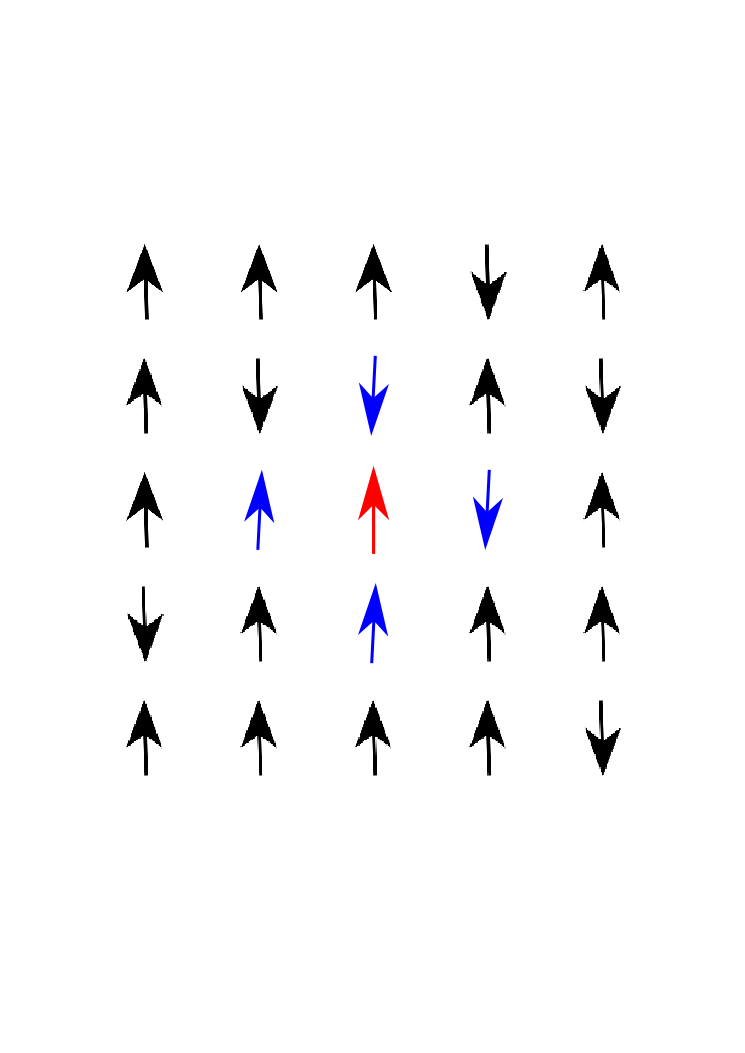
\includegraphics[width=8cm]{myspins.png}	
\caption{ A Sample system of a 5x5 lattice of spins pointing up and down}
\end{figure}

The equation for the total energy of a system of spins is 
\begin{equation}
   E= -J\sum_{<ij>} S_i S_j - \si\micro H \sum_{i=1,N} S_i
\end{equation}
and the magnetization of the system is represented by the following equation
\begin{equation}
   M= \si\micro \sum_{i=1,N} S_i
\end{equation}

where J is the exchange energy, $<ij>$ means the nearest neighbouring spins, $\si\micro$ is the magnetic moment and H represents the strength of an external magnetic field.
\par Without an external magnetic field ($H=0$), the total energy of a system of spins is just the sum of the product of neighbouring spins. For example in FIG.1, the energy at the red spin would be the sum of the interaction between the red arrow and each blue one. In Python, to make sure I don't repeat the same interaction twice, I compute the product of the first spin with the second and add it to the product of the second with the third and so on until the $n^{th}$ spin for each row and column. As for the magnetization, I just calculate the sum of all the spins. 

\section{The Monte Carlo Method}
The interesting idea behind the Monte Carlo is that it relies on randomness to solve a problem. For example, to find the energy or the magnetization of a NxN system at a certain temperature, I repeat the Monte Carlo algorithm as many times as possible and evaluate the average energy and magnetization over all the iterations which represent respectively the approximate value of E and M of the system.
\subsection{The Monte Carlo algorithm}
Starting with a random initial system of spins as depicted in FIG 2, I calculate its total energy. Then, I randomly choose a spin $S_i$ from the system and flip it (If the spin was (-1), it becomes (+1) and vice-versa). I re-calculate the new energy of the system with the spin flipped. I use the acceptance probability formula in equation (3) to either accept or reject the flip.

\begin{figure}[htb]
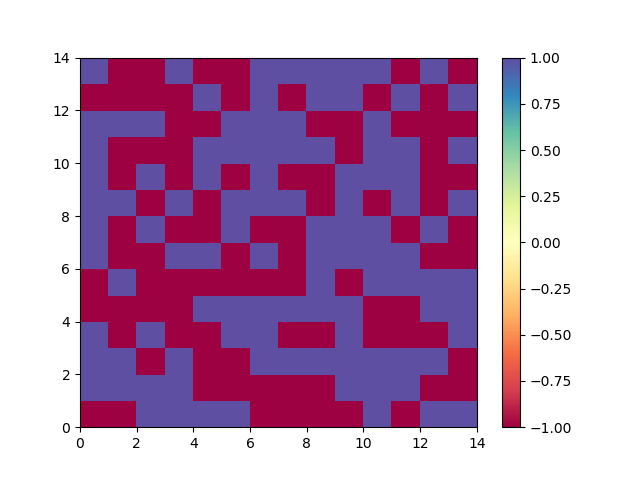
\includegraphics[width=9cm]{initial_spins.png}	
\caption{System of random initial spins of a 15x15 lattice. The purple squares represent the "up" spins and the pink ones represent the "down" spins}
\end{figure}

\begin{equation}
Pa= \left\{ \begin{array}{ll}
              1 & \mbox{if $\Delta E \leqslant 0 $},\\
              e^{-\Delta E/T} & \mbox{if $\Delta E \geqslant 0 $}.\end{array} \right.
\end{equation}
which means that if the change of energy from the initial state to the state with the flipped spin is positive, I accept the flip of the spin with a probability of  $e^{-\Delta E/T}$. 

\par Thus, the final state of spins after many iterations depends on the temperature T. We could notice this difference of final states between T=1 and T=4 in FIG.3 and FIG.4. 
\begin{figure}[htb]
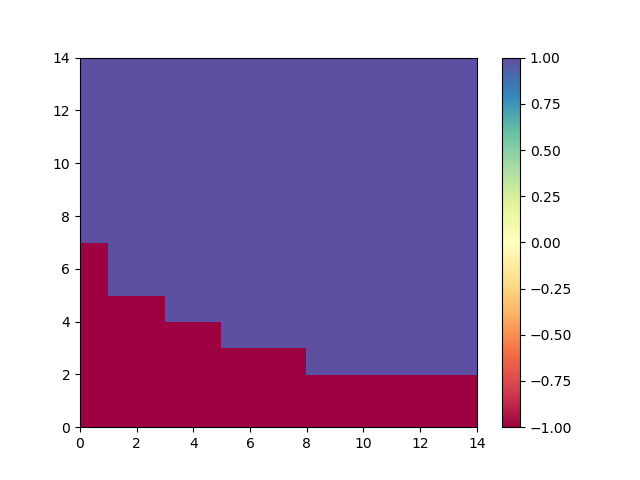
\includegraphics[width=9cm]{final_spins.png}	
\caption{This figure represents the final state of spins after 10000 iterations of the Monte Carlo algorithm for a temperature of T=1}
\end{figure}
\begin{figure}[htb]
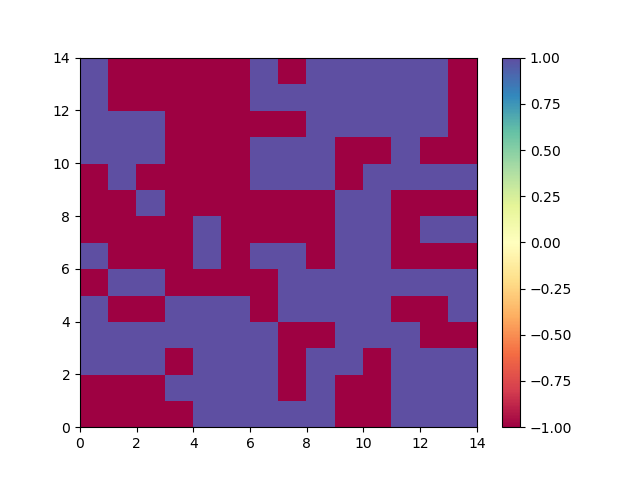
\includegraphics[width=9cm]{final_spins4.png}	
\caption{This figure represents the final state of spins after 10000 iterations of the Monte Carlo algorithm for a temperature of T=4}
\end{figure}

\subsection{Behavior of Energy and Magnetization}
To obverse closely the change of the state of spins as the Monte Carlo algorithm is repeated, I plotted the energy and magnetization as a function of iterations which is represented in FIG.5 and FIG.6. For a temperature T=1, we notice that the energy, after approximately 20000 iterations, stabilizes at value of E= -410 and the magnetization at a value of M= 210. However, for higher temperatures, the model behaves differently. In FIG.7 and FIG.8, for a temperature T=4, the energy and magnetization fluctuate over a wide range of values as the iterations increase. 
\begin{figure}[htb]
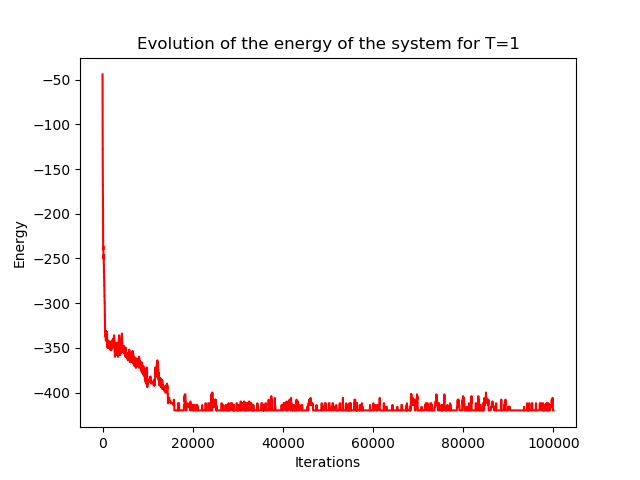
\includegraphics[width=9cm]{E_iteration.png}	
\caption{Change of energy as we iterate the Monte Carlo algorithm for a constant T=1}
\end{figure}
\begin{figure}[htb]
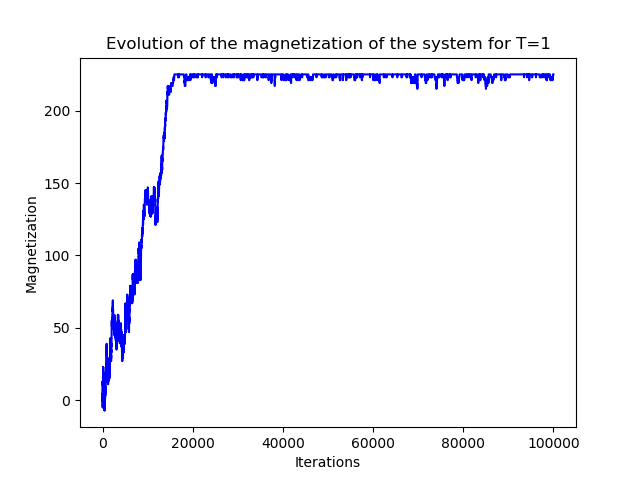
\includegraphics[width=9cm]{M_iteration.png}	
\caption{Change of magnetization as we iterate the Monte Carlo algorithm for a constant T=1}
\end{figure}


\begin{figure}[htb]
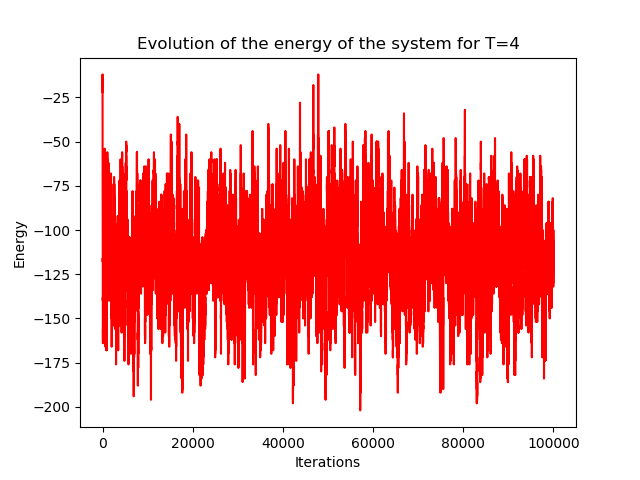
\includegraphics[width=9cm]{E_iteration4.png}	
\caption{Change of energy as we iterate the Monte carlo algorithm for a constant T=4}
\end{figure}
\begin{figure}[htb]
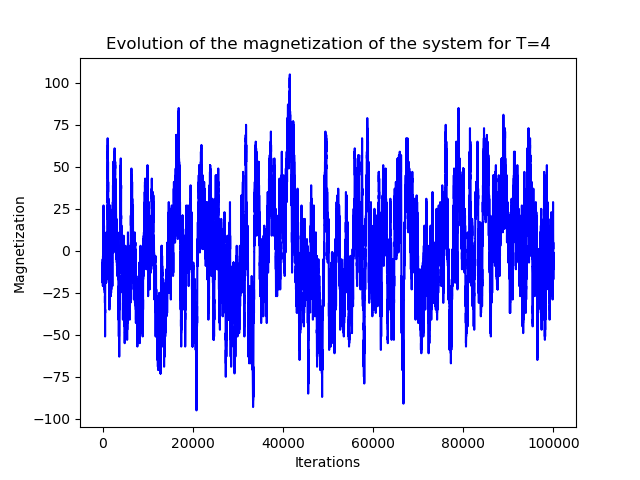
\includegraphics[width=9cm]{M_iteration4.png}	
\caption{Change of magnetization as we iterate the Monte Carlo algorithm for a constant T=4}
\end{figure}



\section{Results}
\subsection{Varying the temperature}
\par As noted in the previous section, the behavior of the Ising model depends on the temperature. That is why I calculated the average energy of all the iterations for each temperature to understand the effect of the temperature on the model. In FIG.9 and FIG.10, we notice that around $T \simeq 2.2$ there is a sudden change in magnetization and energy which represents the phase transition. The temperature at that phase transition is called the critical temperature $T_c$. 
\begin{figure}[htb]
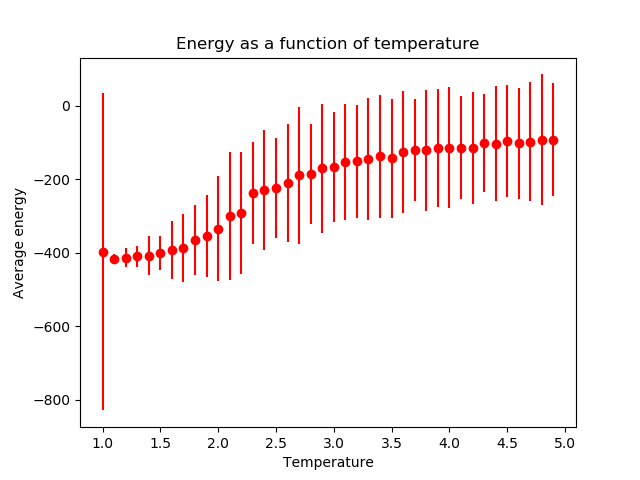
\includegraphics[width=9cm]{E_Temperature.png}	
\caption{Change of energy of the system as we change the temperature}
\end{figure}

\begin{figure}[htb]
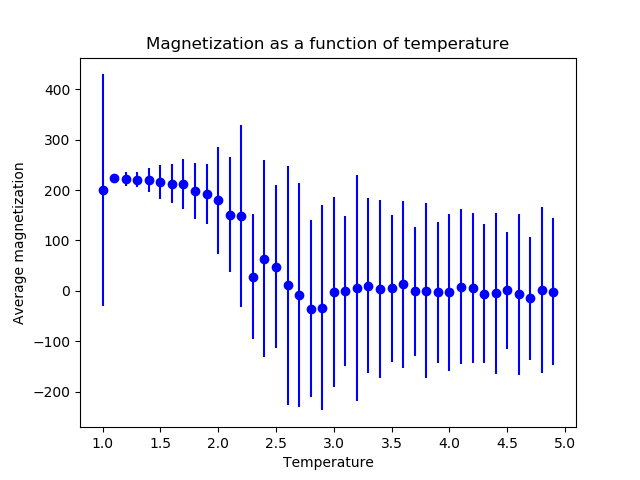
\includegraphics[width=9cm]{M_Temperature.png}	
\caption{Change of magnetization of the system as we change the temperature}
\end{figure}
\par Branislav K. Nikolić published similar results as the ones I got. FIG. 10 and FIG.11 both show the change of magnetization as the temperature increases. In the two plots, the critical temperature is at approximately 2.2. 
\begin{figure}[htb]
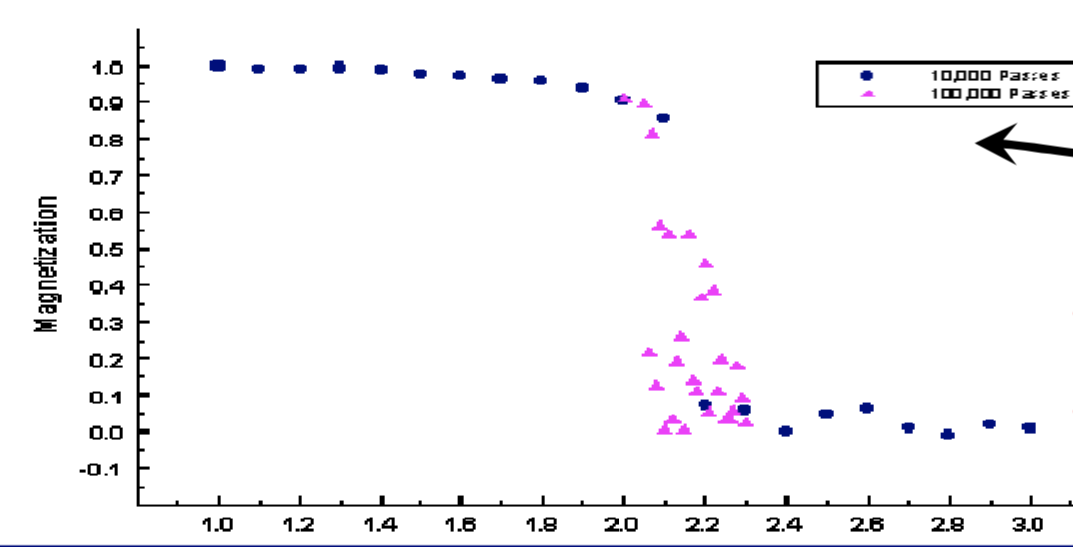
\includegraphics[width=9cm]{test.png}	
\caption{Plot of change of magnetization as a function of temperature by Branislav K. Nikolić}
\end{figure}

\subsection{Adding an external magnetic field}
\par The Ising model depends not only on the temperature, but also on the strength of an external magnetic field H. In FIG.12 and FIG.13, we notice that there an obvious phase transition at H=0. In the energy plot, the change in energy is linear for positive and negative values of H. As for the magnetization plot, the magnetization suddenly shifts from -200 to 200 at H=0. To further my understanding of the behavior of the Ising model when an external magnetic field is present, I re-produced FIG.13 for $T \geqslant T_c$, $T=T_c$ and $T \leqslant T_c$. I expected the plots to shift depending on the temperature. However, surprisingly, the plots didn't change and I couldn't figure out why.
\begin{figure}[htb]
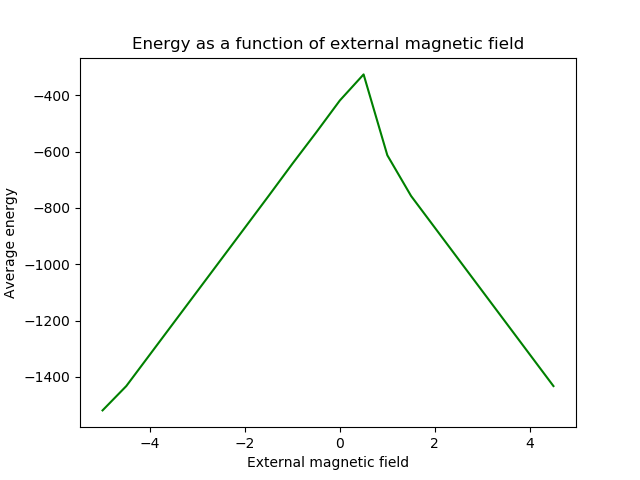
\includegraphics[width=9cm]{E_h.png}	
\caption{Change of energy of the system as we change the external magnetic field for a constant T=1}
\end{figure}

\begin{figure}[htb]
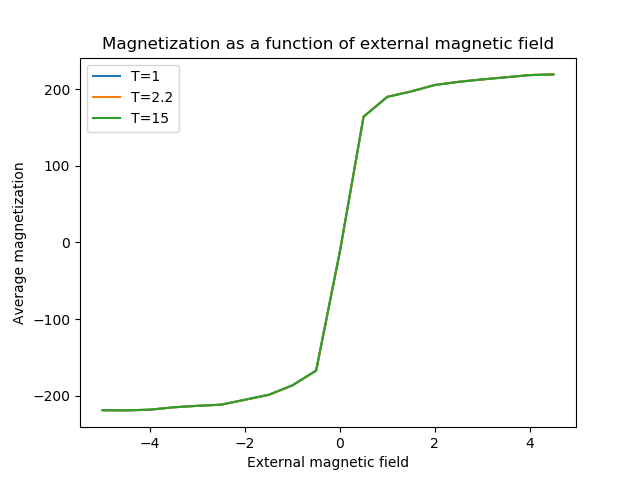
\includegraphics[width=9cm]{E_h_T.png}	
\caption{Change of the magnetization of the system as we change the external magnetic field for T=1, $T=T_c=2.2$ and T=15 }
\end{figure}
\section{Challenges}
\par It is important to acknowledge that working on this project has been extremely rewarding yet challenging in many ways. 
\par One of the challenges I ran into is that my code was computationally expensive. For every 0.1 temperature from T=1 to T=5, I repeat the Monte Carlo algorithm 10000 times and each time the algorithm calls the energy function which has four "for" loops twice. One way I made my code faster is by defining a separate function for the final energy after the spin is flipped. This technique is useful because it uses the initial energy that was already calculated to find the new energy, hence I was able to iterate the Monte Carlo algorithm 100000 times.
\par Another challenge is the plot of magnetization as a function of temperature. The first time I ran my code, it produced FIG.10. However, as I ran it again, I got the same results for the high temperatures ($T \geqslant T_c$), but negative values for low temperatures ($T \leqslant T_c$). 



\section{Reflection}
\par Working on this project has taught a lot. I learned what the Ising model is and how it behaves as the temperature and the strength of an external magnetic field change. I also learned a new, interesting and useful technique which is the Monte Carlo method. 
\par However, due to the time constraint and my limited prior knowledge of the topic, I was not able to thoroughly finish this project. One way, I could have improved this project is by increasing the lattice size to 100X100, exploring more how this topic relates to my previous research and how I could use my results experimentally and doing more research on the strength of the external magnetic field to try to explain why I couldn't notice any change in different temperatures.



\bibliography{ref} 
\nocite{Cipra}
\nocite{Debashish}
\nocite{a}
\nocite{b}
\nocite{c}
\nocite{d}
 
\section*{Acknowledgement}
I would like to acknowledge the great amount of support I received throughout this project. Particularly, I would like to show gratitude to Prof. Daniel Grin for his mentorship, guidance and constructive feedback. I would also like to thank Liam Lynch for giving me an idea of what the Ising model is and sharing his research paper with me. Similarly, I would like to extend my gratitude to my classmates who have contributed greatly to my learning experience throughout the class and especially to the development of my project. 


\end{document} 
